\section{Objectives}
By the end of this laboratory work, students are expected to learn how to 

\begin{itemize}

\item interface mechanical switches with light-emitting diode (LED) circuits and   
  
\item build simple voltage converters (AC to DC) using half-wave and full-wave rectifier circuits that utilize diodes.  
 
  
\end{itemize}

\section{Parts}
\label{sec:partsEx8}
The following parts are required to conduct this laboratory experiment. %
%
\begin{enumerate}
\item Breadboard  
\item One double-pole double-throw (DPDT) switch
\item Two red LEDs
\item Two green LEDs
\item Five 1N5817 (or 1N4148) diodes 
  % \item Five Schottky diodes,  and
\item Four $330~[\ohm]$ resistors
\item Two $10.0~[\kilo\ohm]$ resistors  
\end{enumerate}

\section{Background}
\label{sec:background}

This experiment will highlight the usage of mechanical switches and active electronic devices. The active electronic devices used in this experiment are \emph{diodes} and \emph{light-emitting diodes (LEDs)}.   The mechanical switch will be used to control the operation of independent circuits connected to it. We shall be constructing independent circuits with resistors and LEDs to emulate some applications that will be discussed shortly. Diodes, on the other hand, will be used to construct rectifier circuits that convert AC voltage into DC voltage. In this experiment, we shall focus on constructing simple electronic circuits that emulate the following applications:
%
\begin{enumerate}
    \item Flashing red light,
    \item Traffic light controller using a mechanical switch, and 
    \item Voltage converter (AC to DC).
\end{enumerate}

Before constructing circuits that emulate the above applications, it is important that we review how a mechanical switch, a diode, and an LED work. This is illustrated in the following section. 

\subsection{Mechanical Switch}
In this experiment, we shall consider  a double-pole double-throw (DPDT) switch.  Here, the term ``double-pole'' means two independent switches (also called \emph{commons}) and ``double-throw'' implies two contacts that each independent switch controls. Therefore, a single-pole double-throw (SPDT) switch has a single \emph{common} or \emph{independent switch} and two contacts that it controls. One contact is normally closed and the other contact is normally open. Clearly, a DPDT switch consists of two SPDT switches.  Figure~\ref{fig:DPDT} shows a schematic diagram of a DPDT switch. It consists of two SPDT switches (SPDT~\#1 and SPDT~\#2). Each SPDT switch has a common (see In~\#1 and In~\#2 in Figure~\ref{fig:DPDT}) which is normally closed with one of the output terminals. Therefore, four independent circuits can be connected with four output terminals  (see \emph{Out~\#1a} and  \emph{Out~\#1b} for SPDT\#1, and  \emph{Out~\#2a} and  \emph{Out~\#2b} for SPDT\#2 in Figure~\ref{fig:DPDT}). When the \emph{switch} is in the normally closed (open) position, two circuits are simultaneously active (inactive). A DPDT mechanical switch with the schematic diagram shown in Figure~\ref{fig:DPDT} will be provided for conducting the experiments. 
%

\begin{figure}
  \centering
  \fcolorbox{white}{gray!15}{
    \begin{circuitikz}[scale=1.2]
      \draw
      (0,0) node[anchor=west,spdt](switchSPDT1){~~~{\tiny SPDT\#1}};
      \draw 
      (0,4*\smgrid) node[anchor=west,spdt](switchSPDT2){~~~{\tiny SPDT\#2}};
      % Label each SPDT switch
      \draw
      (switchSPDT1.out 1) node[anchor=west]{Out \#1a};
      \draw
      (switchSPDT1.out 2) node[anchor=west]{Out \#1b};
      \draw
      (switchSPDT1.in) node[anchor=east]{In \#1 (common)};
      \draw
      (switchSPDT2.out 1) node[anchor=west]{Out \#2a};
      \draw
      (switchSPDT2.out 2) node[anchor=west]{Out \#2b};
      \draw
      (switchSPDT2.in) node[anchor=east]{In \#2 (common)};

      \draw[dashed,ultra thick]
      (\smgrid,0.2*\smgrid) -- (\smgrid,5.7*\smgrid)node[anchor=south]{Switch};
    \end{circuitikz}
  }    
  \caption{Schematic diagram of a DPDT switch.}
  \label{fig:DPDT}
\end{figure}
%

\subsection{Diode}
\label{sec:diode}

A (semiconductor) diode is a two-terminal (active) electronic device that allows current to flow in one direction. It consists of a \textit{p}-region that contains holes and an \emph{n}-region which contains electrons. These two regions are separated by a \emph{pn} junction.  When the diode is \emph{on}, the current flows from \emph{p}-region to \emph{n}-region. In other words, a diode has low (ideally zero) resistance from the \emph{p}-region to the \emph{n}-region and high (ideally infinite) resistance from the \emph{n}-region to the \emph{p}-region. Figure~\ref{fig:diodeSymbol} shows a circuit symbol used to represent a \emph{pn} junction diode.  
%
\begin{figure}
  \centering
  \begin{circuitikz}[scale=1.2,american voltages]
    \draw
    node[anchor=east]{\emph{p}}(0,0) to[empty diode,v>=~,o-o,fill=blue!50] (5*\smgrid,0) node[anchor=west]{\emph{n}};
  \end{circuitikz}
  \caption{A diode symbol.}
  \label{fig:diodeSymbol}
\end{figure}
%
Note that a minimum of approximately $V_B = 0.7~[\si{\volt}]$ (called the
``barrier potential'') is required for a silicon diode to be \emph{on}. A diode
is said to be \emph{forward-biased (on)} when the voltage applied to its
terminals is greater than or equal to the barrier potential. Otherwise, the
diode is in the \emph{reverse-biaseded} condition, \textit{i.e.,} no current
flows from the \emph{n}-region to the \emph{p}-region. In this laboratory
experiment, 1N5817 diodes\footnote{See the datasheet provided by the
  manufacturer.} will be used. %; its datasheet can be found at
%\url{http://www.onsemi.com/pub/Collateral/1N4001-D.PDF}, for reference.

\subsection{Light-Emitting Diode (LED)}
\label{sec:light-emitting-diode}
A light-emitting diode (LED) is also a two-terminal electronic device. The main
component of an LED is a semiconductor diode element, typically made of
\emph{gallium arsenide (GaAs)} or \emph{gallium arsenide phosphide (GaAsP)}. It
emits light when a forward-biased voltage is applied across its terminals. An
LED and its circuit symbol are shown in
Figure~\ref{fig:LED-Image}~and~\ref{fig:LED-Symbol}, respectively. The positive
and negative terminals of an LED are the \emph{anode} and \emph{cathode},
respectively. In most cases, \textbf{the longer leg of the LED is the \emph{Anode} while
the shorter leg is the \emph{Cathode}}. Note that the reverse-bias voltage must
be less than $V_{\text{reverse}}=5~[\volt]$ and the continuous forward-bias
current must be less than or equal to $I_{\text{forward}}=25~[\milli\ampere].$ %
%
\begin{figure}
  \centering
  \subfigure[][]{
  \label{fig:LED-Image}
  \begin{tikzpicture}
  \node[inner sep=0pt]{\includegraphics[angle=90]{figs/img/labs/redLED.png}};
  \draw[->]
  (5*\smgrid,1.5)node[anchor=south]{Cathode} -- (5*\smgrid,0.1);
  \draw[->]
  (5*\smgrid,-3*\smgrid)node[anchor=north]{Anode} -- (5*\smgrid,-1.5*\smgrid);
  \end{tikzpicture}
  }
%   \subfigure[][]{
%     \includegraphics[angle=90]{figs/img/labs/redLED.png}
%   }
  \subfigure[][]{
    \label{fig:LED-Symbol}
  \begin{circuitikz}[xscale=1.2,yscale=0.8,american voltages]
    \draw
    node[anchor=east]{Anode}(0,0) to[full led,v>=~,o-o](5*\smgrid,0)node[anchor=west]{Cathode};
  \end{circuitikz}
  }
  \caption{A light-emitting diode.}
  \label{fig:LED}
\end{figure}
%


\section{Working with LEDs}
\label{sec:workingWithLEDs}
We now illustrate how to work with LEDs and interface them with a mechanical DPDT switch. For that, we consider implementing circuits that emulate two simple applications: (1) Flashing red light at an intersection of roads and (2) traffic light controller at an intersection of two one-way roads as illustrated in the following sections. 

\subsection{Flashing Red Light}
\label{sec:FlashingRedLight}
In this part, we shall implement a flashing red light at an intersection of roads on the  breadboard using a function generator that generates a square wave at a frequency of $f.$  The circuit diagram that implements this flashing red light function is shown in Figure~\ref{fig:flashingLED}.  A square wave voltage $v_s(t)$ for $t\ge 0$ with a peak-to-peak voltage of $V_{\text{pp}}~[\si{\volt}]$ is applied to a resistor $R$ with an LED connected in series. The LED is supposed to turn on and off at the frequency of the input signal $v_s(t).$ %
%
\begin{figure}
    \centering
    \begin{circuitikz}[scale=1.2,american voltages]
    \draw 
    (0,0) to[sqV,v<=$v_s(t)$,fill=green!50] (0,4*\smgrid) to[R,v>=$R$](5*\smgrid,4*\smgrid) to[full led,o-o,l^=~~~LED (Red),v>=~](5*\smgrid,0) to[short,-*] (0,0) node[ground]{};
    \end{circuitikz}
    \caption{Circuit for emulating a flashing light.}
    \label{fig:flashingLED}
\end{figure}
%




\subsection{Traffic Light Controller}
\label{sec:voltageDivider}
In this part, we will implement a simple traffic light controller on a breadboard, where the operation of the traffic lights will be controlled using a DPDT mechanical switch. For simplicity, we will be considering traffic lights at the intersection of two one-way roads: East-West (EW) and North-South (NS) as shown in Figure~\ref{fig:intersection}. Two LEDs are used to indicate the traffic signals for each road: one Green and one Red. At any given time, there is an \emph{active direction} with its lights set to green  and an \emph{inactive direction} with its lights set to red. A full light cycle passes through two states as described in Table~\ref{tab:traffic}. %
%
%
% \begin{figure}[h]
%     \centering
%     \includegraphics{figs/ipe/lab7/figure1-intersectionLED.eps}
%     \caption{One-Way Intersection}
%     \label{fig:figure1-intersectionLED}
% \end{figure}
%
%
\begin{figure}
  \centering
  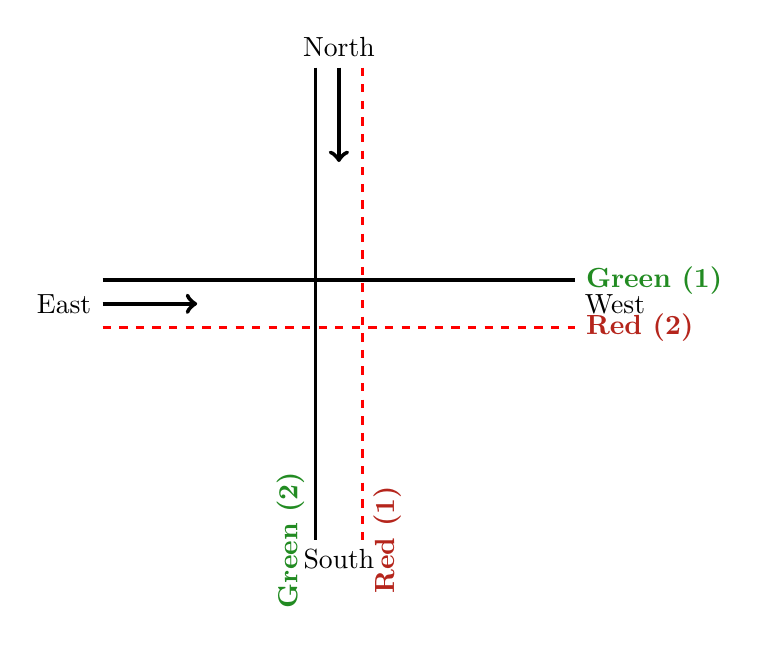
\begin{tikzpicture}[scale=0.6]
    % East-West
    \draw[very thick]
    (-5,0.5) -- (5,0.5)node[anchor=west]{\textcolor{ForestGreen}{\textbf{Green (1)}}};    
    \draw[very thick,red,dashed]
    (-5,-0.5) -- (5,-0.5)node[anchor=west]{\textcolor{BrickRed}{\textbf{Red (2)}}};
    \draw[ultra thick,->]
    (-5,0)node[anchor=east]{East} --(-3,0);
    \draw
    (5,0) node[anchor=west]{West};

    % North-South
    \draw[very thick]
    (-0.5,5) -- (-0.5,-5)node[anchor=south,rotate=90]{\textcolor{ForestGreen}{\textbf{Green (2)}}};    
    \draw[very thick,red,dashed]
    (0.5,5) -- (0.5,-5)node[anchor=north,rotate=90]{\textcolor{BrickRed}{\textbf{Red (1)}}};
    \draw[ultra thick,->]
    (0,5)node[anchor=south]{North} --(0,3);
    \draw
    (0,-5) node[anchor=north]{South};
  \end{tikzpicture}
  \caption{Intersection of two one-way roads.}
  \label{fig:intersection}
\end{figure}

% \subsubsection{Description}
% Consider the traffic lights at the intersection of two roads: East-West and North-South. 
\begin{table}%[htbp]
\caption{Traffic light cycle.}
\label{tab:traffic}
\centering
\begin{tabular}{c|c|c}
\toprule
Direction & EW (1)  & NS (2)\\
\toprule
Active (\textcolor{ForestGreen}{Green}, \textcolor{BrickRed}{Red}) & (1, 0) & (1, 0)\\
\hline
Inactive (\textcolor{ForestGreen}{Green}, \textcolor{BrickRed}{Red}) & (0, 1) & (0, 1)\\
\bottomrule
\end{tabular}

\end{table}

The circuit that emulates this operation of the traffic lights in an intersection of two one-way roads is shown in Figure~\ref{fig:TLC}. Without loss of generality, the DPDT switch is positioned such that the East-West road is in the active mode and the North-South road is in the inactive mode. The operating condition is reversed when the opposite position of the switch is selected.    
%
\begin{figure}
  \centering
  \fcolorbox{white}{gray!15}{
    \begin{circuitikz}[scale=.9, american voltages]
      \tikzstyle{every node} = [font=\tiny]
      \draw 
      (0,4*\smgrid) to[V,l_=$V_s$] (0,0);
      \draw 
      (0,4*\smgrid) -- (4*\smgrid,4*\smgrid)node[anchor = west,spdt](switchSPDT1){~~~\tiny{SPDT~\#1}};
      \draw 
      (switchSPDT1.out 1) to[R,l=$R$,-o] (16*\smgrid,4.6*\smgrid) to[full led,l^=~~\tiny{Red (NS)}](16*\smgrid,0) to[short,-*](0,0)node[ground]{};
      \draw
      (switchSPDT1.out 2) to[R,l=$R$,-o] (12*\smgrid,3.5*\smgrid) to[full led,l_=\tiny{Red (EW)}](12*\smgrid,0);
      
      \draw 
      (4*\smgrid,10*\smgrid)node[anchor = west,spdt](switchSPDT2){~~~\tiny{SPDT~\#2}};
      \draw
      (switchSPDT2.out 1) to[R,l=$R$](20*\smgrid,10.6*\smgrid) to[full led,l^=~~\tiny{Green (EW)},-*](20*\smgrid,7*\smgrid)node[ground]{};
      \draw
      (switchSPDT2.out 2) to[R,l=$R$](12*\smgrid,9.5*\smgrid) to[full led,l^=~~\tiny{Green (NS)}](12*\smgrid,7*\smgrid) --(20*\smgrid,7*\smgrid);

      \draw
      (switchSPDT2.in) to[short,*-*] (switchSPDT1.in);
      
      \draw[dashed,ultra thick]
      (5.2*\smgrid,4.2*\smgrid) -- (5.2*\smgrid,11*\smgrid) node[anchor=south]{Switch};
    \end{circuitikz}
  } % fcolorbox    
    \caption{Circuit for emulating a simple traffic light controller for a one-way intersection.}
    \label{fig:TLC}
\end{figure}




\section{Voltage Converters}
\label{sec:voltageConverters}
In this experiment, we consider voltage converter circuits that convert an AC voltage into a nearly DC voltage. The simplest voltage converters (AC-to-DC) are implemented using rectifier circuits. There are two types of rectifier circuits considered in this experiment: (i) Half-wave rectifier and (ii) Full-wave bridge rectifier. A half-wave rectifier circuit with a resistive load is shown in Figure~\ref{fig:halfWaveRectifier}. When the source voltage $v_s(t)$ is positive (negative), the diode is in the forward (reverse)-biased condition. Let the source voltage $v_s(t)$ be given by $v_s(t) = V_s\sin(\omega t)$ with the angular frequency $\omega = 2\pi f,$ where $f$ is the frequency in $[\hertz],$ $V_s$ is the maximum amplitude, and the time $t\ge 0.$ For an ideal diode, the output voltage across the resistor $R_L$ is given by %
%
\begin{align}
  v_o(t) = \mathrm{max}(0,v_s(t)),
  \label{eq:halfWaveRectifier}
\end{align}
%
where the function $\mathrm{max}(\cdot,\cdot)$ returns the maximum value of its arguments. The average value of the half-wave rectified voltage, $v_{\text{o,avg}}$ is given by %
%
\begin{align*}
    v_{\text{o,avg}} = \frac{V_s}{\pi}.
\end{align*}
%
Note that the average voltage is measured across the load resistor using a digital voltmeter. 
%
\begin{figure}
    \centering
    \begin{circuitikz}[scale=1,american voltages]
      % \tikzstyle{every node} = [font=\tiny]
    \draw 
    (0,0) to[sV,v<=$v_s(t)$,fill=green!50] (0,5*\smgrid)  to[empty diode,v>=~,-*,fill=blue!50] (5*\smgrid,5*\smgrid) to[R,v>=$R_L$,-*](5*\smgrid,0) to[short,-*](0,0) node[ground]{};
    \draw % output wires
    (5*\smgrid,5*\smgrid) to[short,-o](8*\smgrid,5*\smgrid);
    \draw 
    (5*\smgrid,0) to[short,-o](8*\smgrid,0);
    \draw 
    (8*\smgrid,0) to[open,v<=$v_o(t)$](8*\smgrid,5*\smgrid);
    \end{circuitikz}
    \caption{Half-wave rectifier circuit with a resistive load.}
    \label{fig:halfWaveRectifier}
\end{figure}
%
Figure~\ref{fig:fullWaveRectifier} shows a diode bridge circuit that implements a full-wave bridge rectifier. When the source voltage is positive (negative), the diodes $D_1$ and $D_2$ ($D_3$ and $D_4$) are \emph{on}, and the diodes $D_3$ and $D_4$ ($D_1$ and $D_2$) are \emph{off}.  For ideal diodes, the voltage across the load resistor $R_L$ is given by %
%
\begin{align}
  v_o(t) = \big|v_s(t)\big|,
  \label{eq:fullWaveRectifier}
\end{align}
%
and its average value, $v_{\text{o,avg}}$ is given by %
%
\begin{align*}
    v_{\text{o,avg}} = \frac{2V_s}{\pi}.
\end{align*}
%
\begin{figure}
    \centering
    \begin{circuitikz}[scale=1.2,american]
      % \tikzstyle{every node} = [font=\tiny]
      \draw (0,-\smgrid)
      to[sV,v<=$v_s(t)$,fill=green!50] (0,8*\smgrid) -- (8*\smgrid,8*\smgrid)
      to[empty diode,v>=~, l_=$D_1$,fill=blue!50](4*\smgrid,4*\smgrid)
      to[short,-o](5*\smgrid,4*\smgrid)
      to[R,l^=$R_L$,-o,v>=$v_o(t)$](11*\smgrid,4*\smgrid) --
      (12*\smgrid,4*\smgrid) to[empty diode,v>=~,l_=$D_4$,fill=blue!50](8*\smgrid,8*\smgrid);
    
    \draw % lower half
    (8*\smgrid,0) to[empty diode,v>=~,l^=$D_3$,fill=blue!50](4*\smgrid,4*\smgrid);
    \draw
    (12*\smgrid,4*\smgrid) to[empty diode,v>=~,l^=$D_2$,fill=blue!50](8*\smgrid,0);
    \draw 
    (8*\smgrid,0)--(8*\smgrid,-\smgrid) to[short,-*] (0,-\smgrid) node[ground]{};
    \end{circuitikz}    
    \caption{Full-wave rectifier circuit with a resistive load.}
    \label{fig:fullWaveRectifier}
\end{figure}
%
Note, however, that a typical silicon diode requires at least $0.7~[\volt]$ for it to turn on.  

\section{Prelab}
\label{sec:prelab}

The prelab of this experiment is mainly focused on rectifier circuits. It consists of three parts. In the first part, you are to discuss the operating principles of the circuit that emulates the flashing red light at an intersection (see Figure~\ref{fig:flashingLED}) and the traffic light controller circuit shown in Figure~\ref{fig:TLC}. In the second part, you will analyze the half-wave rectifier circuit shown in Figure~\ref{fig:halfWaveRectifier}. In the third part, the effect of full-bridge diode rectifier circuits is observed in converting an AC voltage signal into a nearly DC signal. %
%
\begin{prelab}[LED circuit analysis]{prelab:LED-Circuit}
 Without loss of generality, assume all LEDs are made with ideal diodes. 
 
\begin{enumerate}
    \item Given the circuit shown in Figure~\ref{fig:flashingLED}, where a bi-polar square wave signal $v_s(t)$ with a peak voltage of $V_p$ is applied.  Sketch the input $v_s(t)$ and the output (voltage across resistor $R)$ $v_R(t)$ voltage waveforms.
      \begin{center}
          \begin{tikzpicture}[scale=1]
            \draw[step=0.2cm,gray,very thin](-5*\smgrid,-5*\smgrid) grid (25*\smgrid,5*\smgrid);
            % draw x axis
            \draw[thick,->] (0,0*\smgrid) -- (20*\smgrid,0*\smgrid) node[anchor = north west]{Time $t~[\second]$};
             % draw y axis
            \draw[thick,<->](0,-4*\smgrid) -- (0,5*\smgrid) node[anchor=north east]{Amplitude~$[\volt]$};
          \end{tikzpicture}    
      \end{center}      
      \item Suppose the position of the switch in Figure~\ref{fig:TLC} can be changed between two positions corresponding to the two directions of the intersection of two one-way roads. Briefly discuss the operations (three to five sentences maximum) of Figure~\ref{fig:TLC} when the switch position is interchanged between its two positions.     
\end{enumerate}
\end{prelab}


\begin{prelab}[Half-wave rectifier circuit]{prelab:halfWaveRectifier}
  %
Given the circuit shown in Figure~\ref{fig:halfWaveRectifier} with $v_s(t) = 2.5\sin(2000\pi t)~[\volt],$ and $R = 10~[\kilo\ohm].$ 
      \begin{enumerate}
      \item Using Matlab, show the input and output waveforms, $v_s(t)$ and $v_o(t),$ in one plot for time ranging from $t=0$ to $t=0.01~[\second]$ assuming an ideal diode. [\emph{Hint: Use Equation~\eqref{eq:halfWaveRectifier} to compute the output waveform $v_o(t)$.}]
        
      \item Determine the peak output voltage, $V_p,$ across the load resistor $R_L$ and the average voltage, $v_{\mathrm{o,avg}},$ when a standard silicon diode is used to construct the half-wave rectifier circuit.           
        \end{enumerate}
      \end{prelab}
      
\begin{prelab}[Full-wave bridge  rectifier circuit]{prelab:fullWaveRectifier}
  %
Given the circuit shown in Figure~\ref{fig:fullWaveRectifier} with $v_s(t) = 2.5\sin(2000\pi t)~[\volt],$ and $R = 10~[\kilo\ohm].$ 
      \begin{enumerate}
      \item Using Matlab, show the input and output waveforms, $v_s(t)$ and $v_o(t),$ in one plot for time ranging from $t=0$ to $t=0.01~[\second]$ assuming an ideal diode. [\emph{Hint: Use Equation~\eqref{eq:fullWaveRectifier} to compute the output waveform $v_o(t)$.}]
        
      \item Determine the peak output voltage, $V_p,$ across the load resistor $R_L$ and the average voltage, $v_{\mathrm{o,avg}},$ when a standard silicon diode is used to construct the full-wave rectifier circuit. 
        \end{enumerate}
        
\end{prelab}


\section{Laboratory Work}
\subsection{Part~1}
\label{sec:part1}
\begin{enumerate}

 
\item Measure the value of the $330~[\ohm]$ resistor $(R).$ Then, complete the following table.
%
% 330 Ohm resistor is chosen because the our LEDs can tolerate maximum of 25 [mA] of current. There is approximately 2 [V] drop across an LED. Therefore, 5-15 [mA] current we can pass through the LED. If 5 [V] is applied across an LED then once choice of the resistance connected in series could be R= 330 [Ohm] because   i_d = (5-2)/(330) = 9 [mA] < 25 [mA] 
%
  \begin{center}
    \begin{tabular}{c|c|c}
      \toprule
      Quantity &  Typical & Measured\\
      \toprule
      $R$ & $\ldots$ & $\ldots$\\   %|| R = 
      \bottomrule
    \end{tabular}    
  \end{center}
  
\item Construct the circuit shown in Figure~\ref{fig:flashingLED} using the resistor measured in the previous step and a red LED. 

\item  Using the function generator at your workstation, apply a $0.5~[\hertz]$ bi-polar square wave signal with the  peak amplitude of $V_p = 4~[\volt].$  % V_p = 4 [V] is chosen because reverse-biased voltage of the LED is 5 [V]. 

\item Observe the behavior of the LED and write your observations. 

\item Draw the output voltage waveform, $v_R(t),$  across the resistor $R.$ 
    

  \begin{center}
      \begin{tikzpicture}
        \draw[step=0.2cm,gray,very thin](-5*\smgrid,-5*\smgrid) grid (25*\smgrid,5*\smgrid);
        % draw x axis
        \draw[thick,->] (0,-4*\smgrid) -- (20*\smgrid,-4*\smgrid) node[anchor = north west]{Time $t~[\second]$};
         % draw y axis
        \draw[thick,->](0,-4*\smgrid) -- (0,5*\smgrid) node[anchor=north east]{$v_R(t)$};
      \end{tikzpicture}    
  \end{center}
   
\end{enumerate}

\subsection{Part~2}
\label{sec:part2}
\begin{enumerate}
\item Construct the circuit shown in Figure~\ref{fig:TLC} with $R=330~[\ohm]$ resistors, one DPDT switch, and four LEDs with the appropriate LED colors. 
  
\item Using the DC power supply at your workstation, apply $V_s = 4~[\volt]$ DC voltage and write your observations.
  
\item Test both active and inactive directions of the one-way intersection shown in Figure~\ref{fig:intersection} using the circuit in Figure~\ref{fig:TLC} and write your observations in the Table below. 

  \begin{center}
    \begin{tabular}{c|c|c}
      Direction & EW (1)  & NS (2)\\
      \toprule
      Active (\textcolor{ForestGreen}{\textbf{Green}}, \textcolor{BrickRed}{\textbf{Red}}) & & \\
      \hline
      Inactive (\textcolor{ForestGreen}{\textbf{Green}}, \textcolor{BrickRed}{\textbf{Red}}) & & \\
      \bottomrule
    \end{tabular}    
  \end{center}
  
 \end{enumerate}

\subsection{Part~3}
\label{sec:part3}
\begin{enumerate}

 
\item Measure the resistance of the $10~[\kilo\ohm]$ resistor $(R_L)$ and the diode turn-on voltage using the digital multimeter at your workstation. The diode turn-on voltage can be measured using the diode testing function available on the digital multimeter. Then, complete the following table.

  \begin{center}
    \begin{tabular}{c|c|c}
      \toprule
      Quantity &  Typical & Measured\\
      \toprule
      $R$ & $\ldots$ & $\ldots$\\   %|| R =
      $D_1$ & $\ldots$ & $\ldots$\\   %|| D_1 =       
      \bottomrule
    \end{tabular}    
  \end{center}
  
\item Construct the circuit shown in Figure~\ref{fig:halfWaveRectifier} using the components measured in the previous step. 

\item  Using the function generator at your workstation, apply the voltage $v_s(t) = 2.5\sin(2000\pi t)$ and observe the input and output waveforms on the oscilloscope.

  \item Sketch the input and output voltage waveforms, $v_s(t)$ and $v_o(t),$ respectively. 
  %
  \begin{center}
      \begin{tikzpicture}
        \draw[step=0.2cm,gray,very thin](-5*\smgrid,-5*\smgrid) grid (25*\smgrid,5*\smgrid);
        % draw x axis
        \draw[thick,->] (0,0*\smgrid) -- (20*\smgrid,0*\smgrid) node[anchor = north west]{Time $t~[\second]$};
         % draw y axis
        \draw[thick,<->](0,-4*\smgrid) -- (0,5*\smgrid) node[anchor=north east]{Amplitude~$[\volt]$};
      \end{tikzpicture}    
  \end{center}
  
\item Measure the average output voltage $v_{\mathrm{o,avg}}(t)$ using the digital multimeter at your workstation and record the measure value in the Table below:
  \begin{center}
    \begin{tabular}{c|c|c}
      \toprule
      Quantity &  Computed & Measured\\
      \toprule
      $v_{\mathrm{o,avg}}$ & $\ldots$ & $\ldots$\\
      \bottomrule
    \end{tabular}    
  \end{center}
   
\end{enumerate}


\subsection{Part~4}
\label{sec:part4}
\begin{enumerate}
 
\item Measure the value of the $10~[\kilo\ohm]$ resistor $(R_L)$ and the diode turn-on voltages using the digital multimeter at your workstation. The diode turn-on voltage can be measured using the diode testing function available on the digital multimeter. Then, complete the following table.
%
  \begin{center}
    \begin{tabular}{c|c|c}
      \toprule
      Quantity &  Typical & Measured\\
      \toprule
      $R$ & $\ldots$ & $\ldots$\\   %|| R =
      $D_1$ & $\ldots$ & $\ldots$\\   %|| D_1 =
      $D_2$ & $\ldots$ & $\ldots$\\   %|| D_2 =
      $D_3$ & $\ldots$ & $\ldots$\\   %|| D_3 =
      $D_4$ & $\ldots$ & $\ldots$\\   %|| D_4 =             
      \bottomrule
    \end{tabular}    
  \end{center}
  
\item Construct the circuit shown in Figure~\ref{fig:fullWaveRectifier} using the components measured in the previous step. 

\item  Using the function generator at your workstation, apply the voltage $v_s(t) = 2.5\sin(2000\pi t)$ and observe the input and output  waveforms on the oscilloscope.

\item Sketch the input and output voltage waveforms, $v_s(t)$ and $v_o(t),$ respectively.
  %
  \begin{center}
      \begin{tikzpicture}
        \draw[step=0.2cm,gray,very thin](-5*\smgrid,-5*\smgrid) grid (25*\smgrid,5*\smgrid);
        % draw x axis
        \draw[thick,->] (0,0*\smgrid) -- (20*\smgrid,0*\smgrid) node[anchor = north west]{Time $t~[\second]$};
         % draw y axis
        \draw[thick,<->](0,-4*\smgrid) -- (0,5*\smgrid) node[anchor=north east]{Amplitude~$[\volt]$};
      \end{tikzpicture}    
  \end{center}
  
\item Measure the average output voltage $v_{\mathrm{o,avg}}(t)$ using the digital multimeter at your workstation and record the measure value in the Table below.
  \begin{center}
    \begin{tabular}{c|c|c}
      \toprule
      Quantity &  Computed & Measured\\
      \toprule
      $v_{\mathrm{o,avg}}$ & $\ldots$ & $\ldots$\\
      \bottomrule
    \end{tabular}    
  \end{center}  


   
\end{enumerate}
 

%%% Local Variables:
%%% mode: latex
%%% TeX-master: "../../labBookMechatronics-V2"
%%% End:
